

\documentclass{article}
\usepackage{graphicx}

\begin{document}

\title{Using the concept of informative genomic segment to investigate 
microbial diversity of metagenomics sample}
\author{TBD}
\maketitle
\tableofcontents
\begin{abstract}
\end{abstract}

\section{Introduction}

In almost all  metagenomics projects, diversity analysis plays an important
role to supply information about the richness of species, the species abundance
distribution in a sample or the similarity and difference between different 
samples, all of which are crucial to draw insightful and reliable conclusion. 
Traditionally especially for amplicon metagenomics data set, OTUs(Operational 
Taxonomic Units) based on 16S rRNA genes are used as the basic units for 
diversity analysis. OTUs can be good replacement of the concept of "species" in 
metagenomics. Basically contigs are assembled from reads and are "binned" into
OTUs using composition-based or similarity-based approaches. Then the diversity
can be estimated by using the abundance information of the OTUs.

% from proposal, need to be rewritten to be more precise.
Recently there are many more projects generating whole genome shotgun metagenomics data sets. However they are 
mainly used for assembly and annotation purpose. Less attention was paid to diversity measurement
using these whole genome metagenomics data sets. One possible reason is that the whole genome metagenomics
data sets are often with low depth given the high diversity of metagenomics samples compared to 16S rRNA
ampicon metagenomics data set. Assembly and annotation are always challenging with the low depth and lack of 
reference sequences. It is also true for diversity measurement. On the other hand, although with low depth, some whole genome metagenomics 
data sets are with large size because of the high diversity. For instance, there may be 4 petabase
pairs of DNA in a gram of soil{Zarraonaindia:2013aa}. Many of those methods for sequence binning or diversity 
estimation do not scale well and will not work for large metagenomics data sets. For instance,
many composition-based binning approach involves k-mer/signature frequency distribution calculation, which is 
rather computationally expensive. Even basic sequence alignment will be impossible for large metagenomics data set.
Many of those statistical software packages to estimate diversity using various estimators are not prepared 
for the large scale of whole genome metagenomics data. 

With the development of next generation sequencing technology, the cost of sequencing is dropping rapidly. 
Whole genome metagenomics sequencing is more popular and large amount of metagenomics data is 
being generated with increasing speed, which can not be even met by the increase of computational capacity.
Novel methods that can scale well are extremely needed to deal with the increasingly large metagenomics data
set. 


%diversity analysis, is the central topic of in microbial ecology.
%
%
%1. traditionally, OTU 
%
%2. assembly, annotation, 
%megan, 
%
%binning
%
%3. co abundance methods.
%
%4. alpha , genome size estimation.
%
%5. igs, better , advantage
%
%alpha, beta 
%
%
%
%assembly, contig binning
%
%no assembly, no reference sequence
%
%
%kmer couting, 
%
%paper:
%
%alpha, co abundance, 
%beta, co abundance across samples
%
%
%
%
%khmer counting,
%
%streaming, diginorm, 
%


Here we propose a novel concept - IGS (informative genomic 
segment) and use IGS as a replacement of OTUs to be the cornerstone for 
diversity analysis of whole shotgun metagenomics data sets. IGSs represent the 
unique information in a metagenomics data set and the abundance of IGSs in 
different samples can be retrieved by the reads coverage through an efficient 
k-mer counting method. This samples-by-IGS abundance data matrix is a promising
replacement of samples-by-OTU data matrix used in 16S rRNA based analysis and 
all existing statistical methods can be borrowed to work on the samples-by-IGS 
data matrix to investigate the diversity. We applied the IGS-based method to 
several simulated data sets and a real data set - Global Ocean Sampling 
Expedition (GOS) to do beta-diversity analysis and the samples were clustered 
more accurately than existing alignment-based method. We also tried this novel 
method to Great Prairie Soil Metagenome Grand Challenge data sets. Furthermore 
we will show some preliminary results using the IGS-based method for 
alpha-diversity analysis. Since this method is totally binning-free, 
assembly-free, annotation-free, reference-free, it is specifically promising 
to deal with the highly diverse samples, while we are facing large amount of 
“dark matters” in it, like soil.






\section{Results}


\subsection{IGS(informative genomic segment) can represent the novel information of a genome}

Median k-mer abundance can represent sequencing depth of a read(cite diginorm). For a sequencing reads data set with multiple species, the sequencing depth of a read is related to the abundance of species where the read originates. 


The Figure \ref{fig:reads_to_IGS} a shows the abundance distribution with different sequencing depth of reads from 4 simulated sequencing data sets - 3 sequencing data sets generated with different sequencing coverage(1x, 10x, 40x) from 3 simulated random genomes respectively and 1 combined data set with all the previously mentioned data sets. No error is introduced in these simulated data sets. Obviously the reads from the three data sets can be separated by estimated sequencing depth. The combined data set can be considered as a sequencing data set with three species with different abundance.

Each point on the curve shows that there are Y reads with a sequencing depth of X. In other word, for each of those Y reads, there are X-1 other reads that cover the same DNA segment in a genome that single read originates. So we can estimate that there are Y/X distinct DNA segments with reads coverage as X. We term these distinct DNA segments in species genome as IGS(informative genomic segment). We can transform the figure in upper position to show the number of IGSs and their respective reads coverage, as shown in figure in lower position. We sum up the numbers of IGSs with different reads coverage for each data set and get the result as shown in below. The sum numbers of IGSs here essentially are the areas below each curve in the figure.

Even though the datasets have different sequencing depth like 10X and 40X, they have similar numbers of IGSs. Dataset with 1X sequencing depth has fewer IGSs because the depth is not enough to cover all the content of the genome(63.2\%) Essentially it is the maximum number of segments with length L on a genome out of which no two segments share any single k-mer. See Figure below. Assume the species genome is totally random, which is the case in the simulated data set, the number of IGSs(N) in a species genome is related to the size of genome(G), read length(L) and k size(k), which can be denoted as

N =G/(L-k+1)

For the simulated genome with size of 1M bps, read length as 80bps, k-mer size as 22bps,expected number of IGSs is 

1000000/(80 - 22 + 1) = 16949, 

pretty close to observed value. Table \ref{table:IGSs}


\begin{figure}[!ht]
\centerline{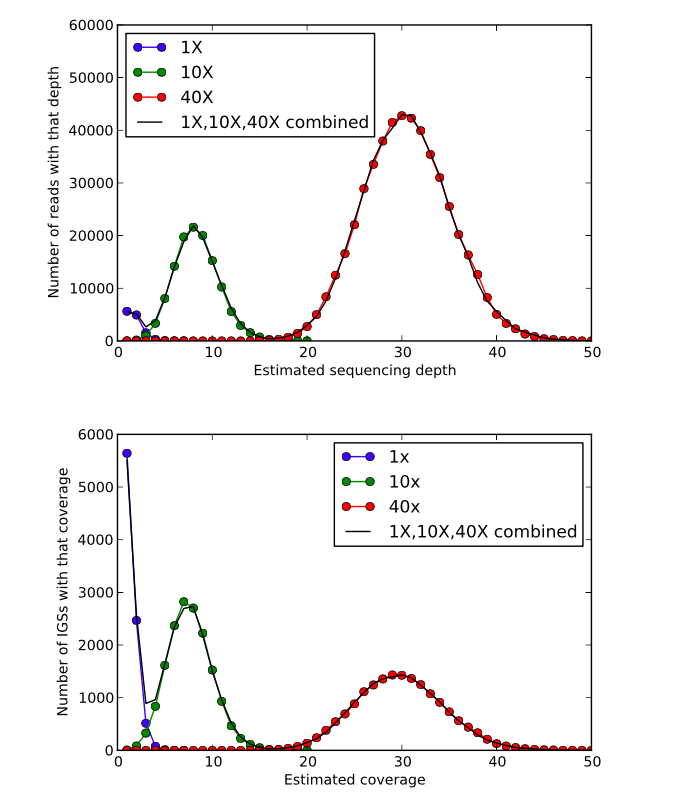
\includegraphics[width=4in]{./figures/from_reads_to_IGS.png}}
%\caption{\bf cluster of GOS samples using IGS method}
\caption{\bf from reads to IGS}
\label{fig:reads_to_IGS}
\end{figure}

\begin{table}[!ht]
\caption{
\bf{Total number of IGSs in different simulated reads data sets.}
}
\begin{tabular}{ |c | c |c| c|c| }
Data set & total number of IGSs \\
\hline \\
1X depth                   & 8714  \\
10X depth                  & 16321  \\
40X depth                  & 16794 \\
1X,10X,40X combined        & 41742 \\
\end{tabular}
\begin{flushleft}
\end{flushleft}
\label{table:IGSs}
\end{table}


\begin{figure}[!ht]
\centerline{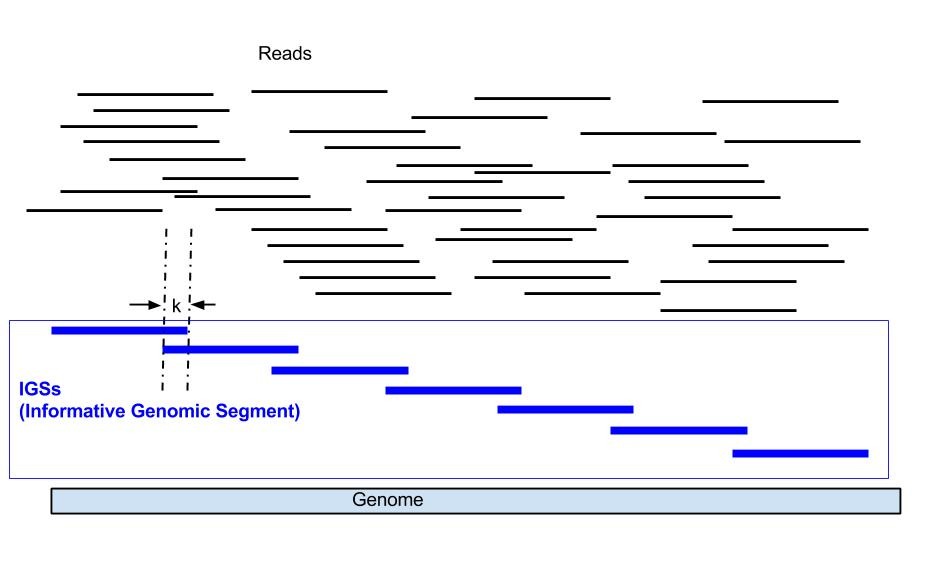
\includegraphics[width=4in]{./figures/IGSs_figure.jpg}}
\caption{\bf the concept of IGS}
\label{fig:IGS}
\end{figure}

\subsection{IGS can be used to do alpha diversity analysis}

Basically the abundance distribution of IGSs with different coverage in a sample data set is acquired using the method shown above, like:

    3 23
    4 24
    5 25
    6 25
    ...

Here 23 IGSs with coverage as 3, this number is calculated from dividing the total number of reads with coverage as 3, which is 69, by the coverage 3: 69/3. Similarly there are 96/4 = 24 IGSs with coverage as 4.

If we draw an analogy between IGSs and OTUs, this is like there are 23 different OTUs with 3 reads mapped to, and 24 different OTUs with 4 reads mapped to. 

Then list all the different IGSs and the corrensponding count,and we can get a long list with each IGS and the corresponding coverage.The coverage of an IGS can be considered as the abundance of such IGS in a sample. The list looks like:

%    #IGS_ID sample_ID
%    1     3
%    2     3
%    3     3
%    ...
%    23    3
%    24    4
%    25    4
%    ...
%    47    4
%    48    5
%    ...
    ...
  
This list is the counterpart of an OTU table in OTU based diversity analysis.

With such table at hand, numerous existing statistical methods and software packages can be used to investigate the alpha diversity.  

In the experiments shown below, QIIME package was used. 




\subsection{IGS can be used to do beta diversity analysis}

As in alpha diversity analysis, OTU table is also a cornestone for beta diversity analysis. As long as we get a reliable OTU table, there are existing pipelines to do the beta diversity analysis. 

A typical OTU table across different samples is like this, which is also called samples-by-OTU data matrix.

%    OTU_ID Sample1_ID Sample2_ID Sample3_ID
%   OTU1   3          4          2
%    OTU2   2          5          0
%    OTU3   3          1          4

    
Like a OTU table, we hope to have the IGS table for the IGSs:

%    IGS_ID SampleA SampleB SampleC SampleD
%    IGS1   5       1       2       1
%    IGS2   5       1       2       1

    
    So now the problem is how we can generate a sample-by-IGS data matrix as the couterpart of samples-by-OTU data matrix so many of  the existing tools/methods used for OTU-based diversity can be borrowed for this kind of IGS-based analysis, just as what is shown above for alpha diversity analysis.

Firstly, as how we get the coverage of a read from a sample dataset in this sample dataset, we can get the coverage of a read from a sample A dataset in another sample B dataset. We can still use the median k-mer count to represent the coverage. The basic idea is the same. 

%Because a read must derive from a segment in the genome of some species in a sample, if a read R from sample A with a coverage C_A in sample A has a coverage as C_B in sample B, that means that segment of genome in sample A from which read R derive also exists in sample B. That genomic segment has a coverage as C_A in sample A and has a coverage as C_B in sample B. Roughly there should be about C_A reads (read R should be one of them) in sampleA covering that genomic segment and C_B reads in sampleB covering that genomic segment. Meanwhile, the C_A reads in sampleA should all have a coverage as C_B in sampleB, just like read R as one of them. Similary, the C_B reads in sampleB should all have a coverage as C_A in sampleA.

Ok, now let's make an example. 

Suppose there are 6 reads in sample A, all have a coverage as 3 in sampleA, and have a coverage as 2 in sampleB.

According to the discussion about IGS in previous section, the 6 reads cover 2 IGSs with a coverage as 3 for each IGSs. There should be 4 reads in sampleB covering the exact same 2 IGSs, with a coverage as 2 in sampleB.

So now we have 2 distinct IGSs with redundancy as 3 and 2 in the two samples respectively. 

**Note:** small number is used in the analysis above as example, but it should be emphasized that the analysis is based on large number statistically.


Let's expand this example from 2 samples to 4 samples(A,B,C,D), as shown in figure above.

Let's say we find 10 reads in sampleA, with coverage as 5-1-2-1 in samples A-B-C-D respectively. (We call "5-1-2-1" "coverage  spectrum" across samples.) So there should be **about** 2 reads in sampleB, 4 reads in sampleC, 2 reads in sampleD, all of which have a "coverage spectrum" as "5-1-2-1". Basically these 18 reads altogether cover 2 distinct IGSs, which apparently exist in all the 4 samples. The 2 distinct IGSs has a redundancy as 5,1,2,1 in the 4 samples respectively.

If we draw an analogy between IGSs and OTUs, this is like there are 2 OTUs, both with 5,1,2,1 reads mapped to in sample A,B,C,D respectively.

Like a OTU table, here we can have the IGS table for the two IGSs:
%
%    IGS_ID SampleA SampleB SampleC SampleD
%    IGS1   5       1       2       1
%    IGS2   5       1       2       1
%    
    
    
 % should all include alpha and beta diversity results
    
\subsection{GOS data sets: Sorcerer II Global Ocean Sampling Expedition}

\paragraph{Using IGS can get comparable cluster of samples:}

Using IGS can get cluster of samples

\begin{figure}[!ht]
 \centerline{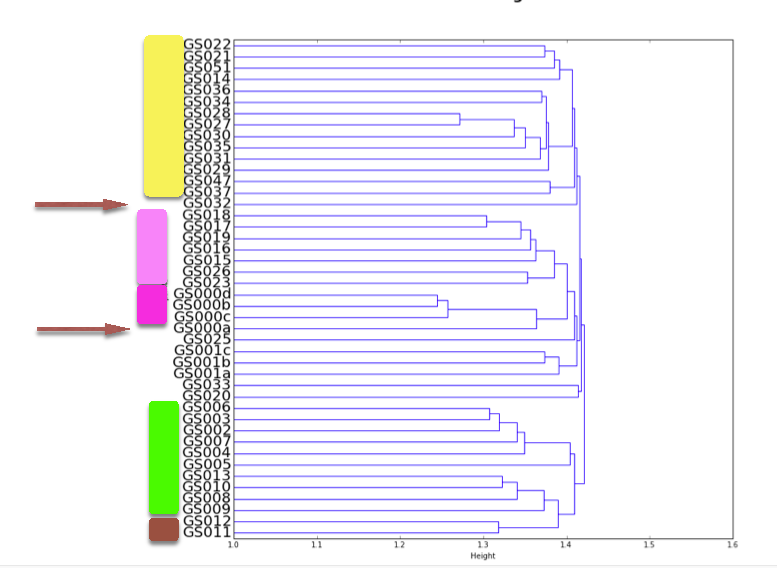
\includegraphics[width=4in]{./figures/GOS_cluster.png}}
\caption{\bf cluster of GOS samples using IGS method}
\label{fig:concept}
\end{figure}

\begin{figure}[!ht]
 \centerline{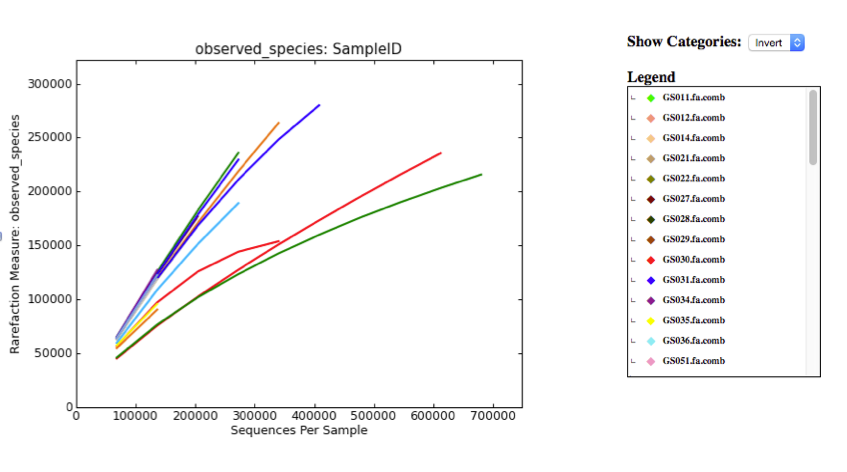
\includegraphics[width=4in]{./figures/GOS_observed.png}}
\caption{\bf cluster of GOS samples using IGS method}
\label{fig:concept}
\end{figure}

\begin{figure}[!ht]
 \centerline{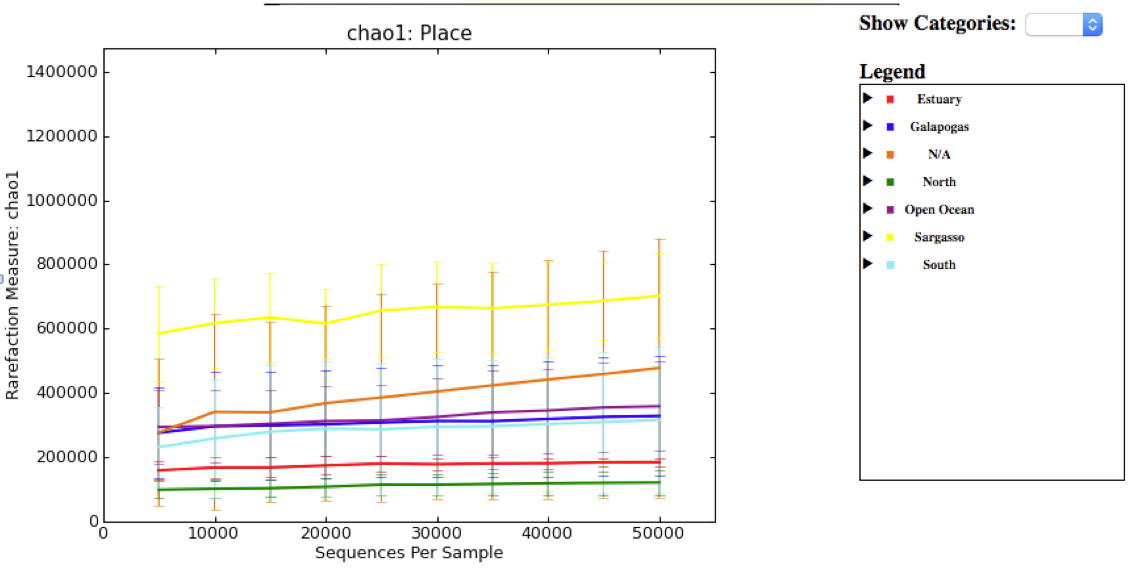
\includegraphics[width=4in]{./figures/GOS_chao.png}}
\caption{\bf cluster of GOS samples using IGS method}
\label{fig:concept}
\end{figure}


% result not good, remove it?
%\subsection{MetHit Human Gut metagenomics data set}


\subsection{HMP metagenomics data set}
% now have alpha and beta, smallest samples
% full sample 110 .... good for binning?

\begin{figure}[!ht]
 \centerline{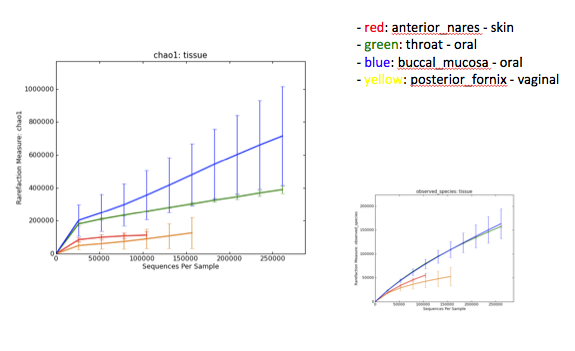
\includegraphics[width=4in]{./figures/HMP_alpha.png}}
\caption{\bf rarefaction of HMP}
\label{fig:concept}
\end{figure}

\begin{figure}[!ht]
 \centerline{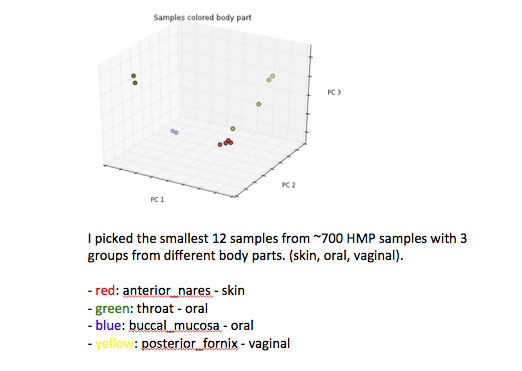
\includegraphics[width=4in]{./figures/HMP_beta.png}}
\caption{\bf PCoA of HMP}
\label{fig:concept}
\end{figure}



% ARMO subset 1m, Gpgc only 1m/2m subset, scalable??
\subsection{GPGC soil sample - new and old}

%new GPGC has better understanding??

% should be enough??

Using 1m and 2m randomly selected subsets can yield pretty good results.



\begin{figure}[!ht]
 \centerline{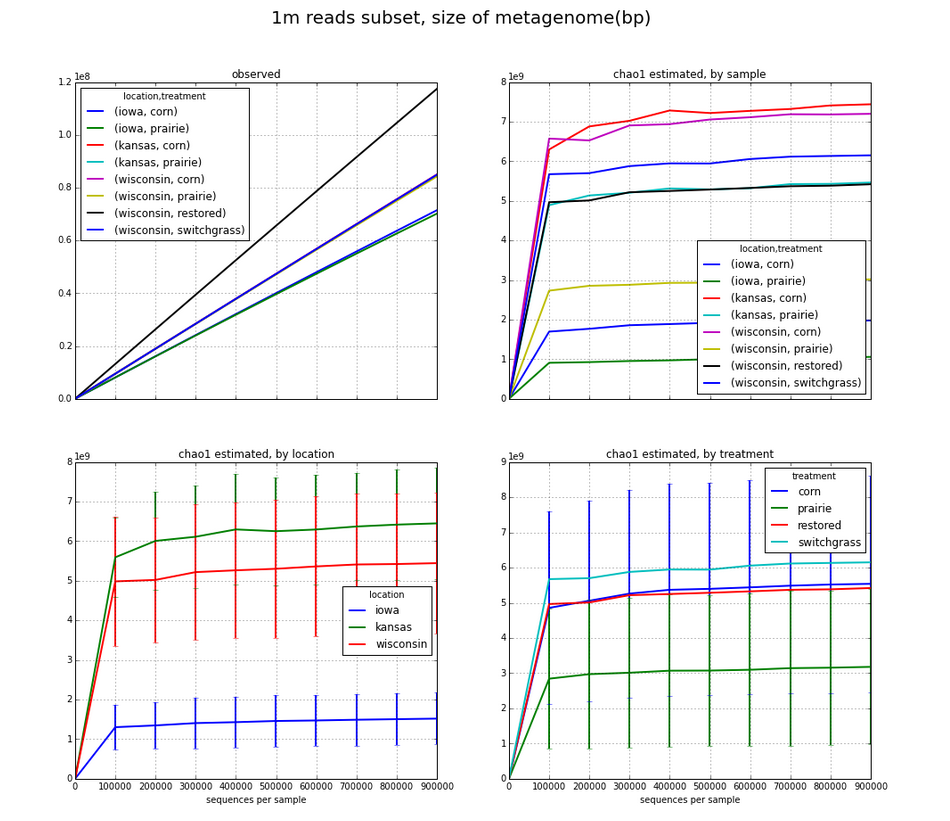
\includegraphics[width=4in]{./figures/GPGC_1m_old.png}}
\caption{\bf alpha of GPGC}
\label{fig:concept}
\end{figure}



\begin{figure}[!ht]
 \centerline{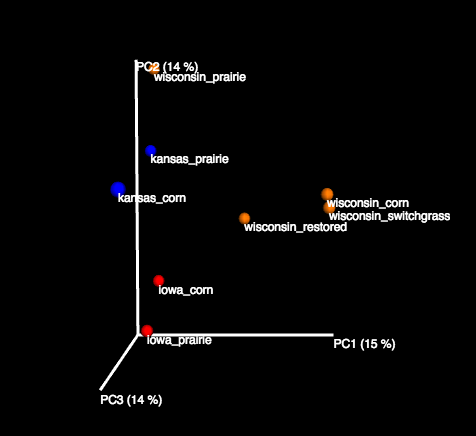
\includegraphics[width=4in]{./figures/GPGC_old_subset1M.png}}
\caption{\bf beta of GPGC}
\label{fig:concept}
\end{figure}

\subsection{iterated diversity analysis}

As we load more reads, we will see the separation more clearly. 

simulated data sets. 



\section{Discussion}

\subsection{IGS can be the foundation of a new framework to do microbial diversity analysis}


\subsection{IGS is promising to more problems}

1. alpha-diversity analysis (1 sample)
    - richness/evenness
    - rarefaction curve
    - sequencing depth evaluation
    - genome size estimation
    - better choosing diginorm parameters(size of hashtables, etc.)

2. beta-diversity (multiple samples)
    - sample by sample comparison, clustering, ordination after getting segment-count table

3. other potential applications:
    - reads binning/classification (after clustering)(if number of samples is small, may not be effective)
    - extract IGS(reads) according different filters (shared by all samples, or some specific samples, )
    - co assembly (by extracting the reads with total coverage across samples > 10, for example)
    
    

\subsection{Concluding thoughts}



\section{Conclusion}
Advantage:

not only HMP, high depth, data
but also low depth data, like soil metagenomics, which is impossible to use traditional method 



\section{Methods}

\subsection{Simulated data sets}

\subsubsection{Four simulated reads data sets with different species abundance distribution}

\subsubsection{Simulated sequencing reads of e.coli}

Here we simulated 4 sequencing reads data sets with read length as 100bp of e.coli with different sequencing depth(50x and 150x) and different sequencing error rate(1\%,2\% and 0\%). Table \ref{table:ecoli}

\begin{table}[h]
\caption{
\bf{Simulated sequencing reads data sets of e.coli}
}
\begin{tabular}{|l|l|l|ll}
\cline{1-3}
sample & coverage & error rate &  &  \\ \cline{1-3}
A      & 150      & 0.01       &  &  \\ \cline{1-3}
B      & 50       & 0.01       &  &  \\ \cline{1-3}
C      & 50       & 0.01       &  &  \\ \cline{1-3}
D      & 50       & 0.02       &  &  \\ \cline{1-3}
\end{tabular}
\label{table:ecoli}
\end{table}



\begin{table}[h]
\caption{GPGC Data sets}
\label{my-label}
\begin{tabular}{|l|l|l|l|l|}
\hline
sample & \# of reads & size of .gz file & \# of bps & ave. length \\ \hline
iowa corn & 1514290825 & 46G & 144202427079 & 95.2 \\ \hline
iowa prairie & 2597093273 & 74G & 226815059143 & 87.3 \\ \hline
kansas\_corn & 2029883371 & 66G & 206933829048 & 101.9 \\ \hline
kansas\_prairie & 0 & 145G & 0 & 0 \\ \hline
wisconsin\_corn & 1616440116 & 51G & 162257698471 & 100.4 \\ \hline
wisconsin\_prairie & 1653557590 & 53G & 166467901724 & 100.7 \\ \hline
wisconsin\_restored & 226830595 & 11G & 34241520930 & 151.0 \\ \hline
wisconsin\_switchgrass & 310966735 & 13G & 40259619921 & 129.5 \\ \hline
\end{tabular}
\end{table}


\subsection{The concept of IGS(informational genomic segment)}

In classic ecology dealing with macroorganisms, diversity measurement is based on the concept of ?species?. For 16S rRNA amplicon metagenomics data set, it is based on the concept of ?OTUs?. When the concept of OTUs does not work for large shotgun metagenomics data set, in the beginning we proposed that the concept of k-mers(a DNA segment with the leng of k) can be used to measure diversity. K-mers can be considered as the atom of information in DNA sequences. One of the composition-based approaches to binning is to use the k-mer as the signature. Suppose the sizes of microbial genomes are similar and the difference between genomic content of microbial genomes is similar, the number of distinct k-mers in the sequence data set is related to the number of species in a sample. However, because of sequencing error, which is unavoidable due to the limit of sequencing technology, this k-mer based analysis doe not work well. One sequencing error on a read will generate at most k erroneous k-mers. In metagenomics data set with low coverage, most of the distinct observed k-mers are from sequencing errors.


Next we turned our gaze to the upper level - reads. A novel method termed as ?digital normalization? was developed to remove abundant reads before assembly. However it also supplies a novel way to distil information from reads by decreasing the bad influence of sequencing errors so that we can use those informative reads to measure the microbial diversity. We term those informative reads as IGS(informative genomic segment), which can be considered as a segment of DNA on a microbial genome. Those IGSs should be different enough to represent the abstract information a genome contains. Suppose microbial genomes contain similar number of those IGSs, as they contain similar number of distinct k-mers, the number of IGSs will be related to the species richness in a sample, and the abundance distribution of IGSs will be related to species evenness in a sample. Many classic diversity estimation methods based on OTUs level described in sections above can be borrowed to estimate the diversity of IGSs and the diversity of actual species subsequently.

IGS may be a good concept in whole genome shotgun metagenomic diversity analysis, especially while facing large amount of "dark matters", unknown species. We don't care about species, we only care about how much information there is in the sample.


For alpha diversity, we can generate a list of IGSs and the respective abundance in a sample. Then existing estimators like Chao's can be used to estimate total number of IGSs in the sample. Rarefaction curve based on number of IGSs can also be generated. 

For beta diversity, here we will generate a samples-by-IGS data matrix, as a replacement of samples-by-OTU data matrix in 16s based analysis and samples-by-species data matrix in traditional ecology. 


From that samples-by-IGS data matrix, we can use existing methods to calculate similarity/disimilarity/distance between samples and do ordination. QIIME and Mother can do this kind of jobs pretty well.

With the samples-by-IGS data matrix, it is also possible to calculate similarity between IGSs and do ordination, which is a potential approach to classify IGS( reads).

Using median k-mer frequency can decrease the influence of sequencing error, but can not eliminate the influence of errors. This can cause some problems in the following analysis, which will be discussed in details.


%Using simulated and real genomic data sets, with the help of khmer to get median k- mer abundance, we find that median k-mer abundance correlates well with mapping-based coverage.

%Side note: We can also see that the coverage by median k-mer count is generally lower than the read coverage by mapping. So estimation of sequencing coverage by median k-mer count is underestimated. This can cause some problems in later analysis, which will be discussed later.

\subsection{Using IGS to do alpha diversity analysis}


Basically the abundance distribution of IGSs with different coverage in a sample data set is acquired using the method shown above, like:

    3 23
    4 24
    5 25
    6 25
    ...

Here 23 IGSs with coverage as 3, this number is calculated from dividing the total number of reads with coverage as 3, which is 69, by the coverage 3: 69/3. Similarly there are 96/4 = 24 IGSs with coverage as 4.

If we draw an analogy between IGSs and OTUs, this is like there are 23 different OTUs with 3 reads mapped to, and 24 different OTUs with 4 reads mapped to. 

Then list all the different IGSs and the corrensponding count,and we can get a long list with each IGS and the corresponding coverage.The coverage of an IGS can be considered as the abundance of such IGS in a sample. The list looks like:

%    #IGS_ID sample_ID
%    1     3
%    2     3
%    3     3
%    ...
%    23    3
%    24    4
%    25    4
%    ...
%    47    4
%    48    5
%    ...
    ...
  
This list is the counterpart of an OTU table in OTU based diversity analysis.

With such table at hand, numerous existing statistical methods and software packages can be used to investigate the alpha diversity.  

In the experiments shown below, QIIME package was used. 



\subsection{Using IGS to do beta diversity analysis}


\section{Acknowledgments}


\end{document}
